\documentclass{article}
\usepackage[utf8x]{inputenc}
\usepackage{ucs}
\usepackage{amsmath} 
\usepackage{amsfonts}
\usepackage{upgreek}
\usepackage[english,russian]{babel}
\usepackage{graphicx}
\usepackage{float}
\usepackage{textcomp}
\usepackage{hyperref}
\usepackage{mathtools}
\usepackage{geometry}
  \geometry{left=2cm}
  \geometry{right=1.5cm}
  \geometry{top=1cm}
  \geometry{bottom=2cm}
\usepackage{tikz}
\usepackage{ccaption}
\usepackage{multicol}
%\setlength{\columnsep}{1.5cm}
%\setlength{\columnseprule}{0.2pt}
\usepackage{listings}

\DeclarePairedDelimiter\ceil{\lceil}{\rceil}
\DeclarePairedDelimiter\floor{\lfloor}{\rfloor}

\begin{document}
\pagenumbering{gobble}

\lstset{
  language=C,                % choose the language of the code
  basicstyle=\linespread{1.1}\ttfamily,
  columns=fixed,
  fontadjust=true,
  basewidth=0.5em,
  keywordstyle=\color{blue}\bfseries,
  commentstyle=\color{gray},
  stringstyle=\ttfamily\color{orange!50!black},
  showstringspaces=false,
  %numbers=false,                   % where to put the line-numbers
  numbersep=5pt,
  numberstyle=\tiny\color{black},
  numberfirstline=true,
  stepnumber=1,                   % the step between two line-numbers.        
  numbersep=10pt,                  % how far the line-numbers are from the code
  backgroundcolor=\color{white},  % choose the background color. You must add \usepackage{color}
  showstringspaces=false,         % underline spaces within strings
  captionpos=b,                   % sets the caption-position to bottom
  breaklines=true,                % sets automatic line breaking
  breakatwhitespace=true,         % sets if automatic breaks should only happen at whitespace
  xleftmargin=.2in,
  extendedchars=\true,
  keepspaces = true,
}
\lstset{literate=%
   *{0}{{{\color{red!20!violet}0}}}1
    {1}{{{\color{red!20!violet}1}}}1
    {2}{{{\color{red!20!violet}2}}}1
    {3}{{{\color{red!20!violet}3}}}1
    {4}{{{\color{red!20!violet}4}}}1
    {5}{{{\color{red!20!violet}5}}}1
    {6}{{{\color{red!20!violet}6}}}1
    {7}{{{\color{red!20!violet}7}}}1
    {8}{{{\color{red!20!violet}8}}}1
    {9}{{{\color{red!20!violet}9}}}1
}

\section*{Хеш-таблицы}

\begin{center}
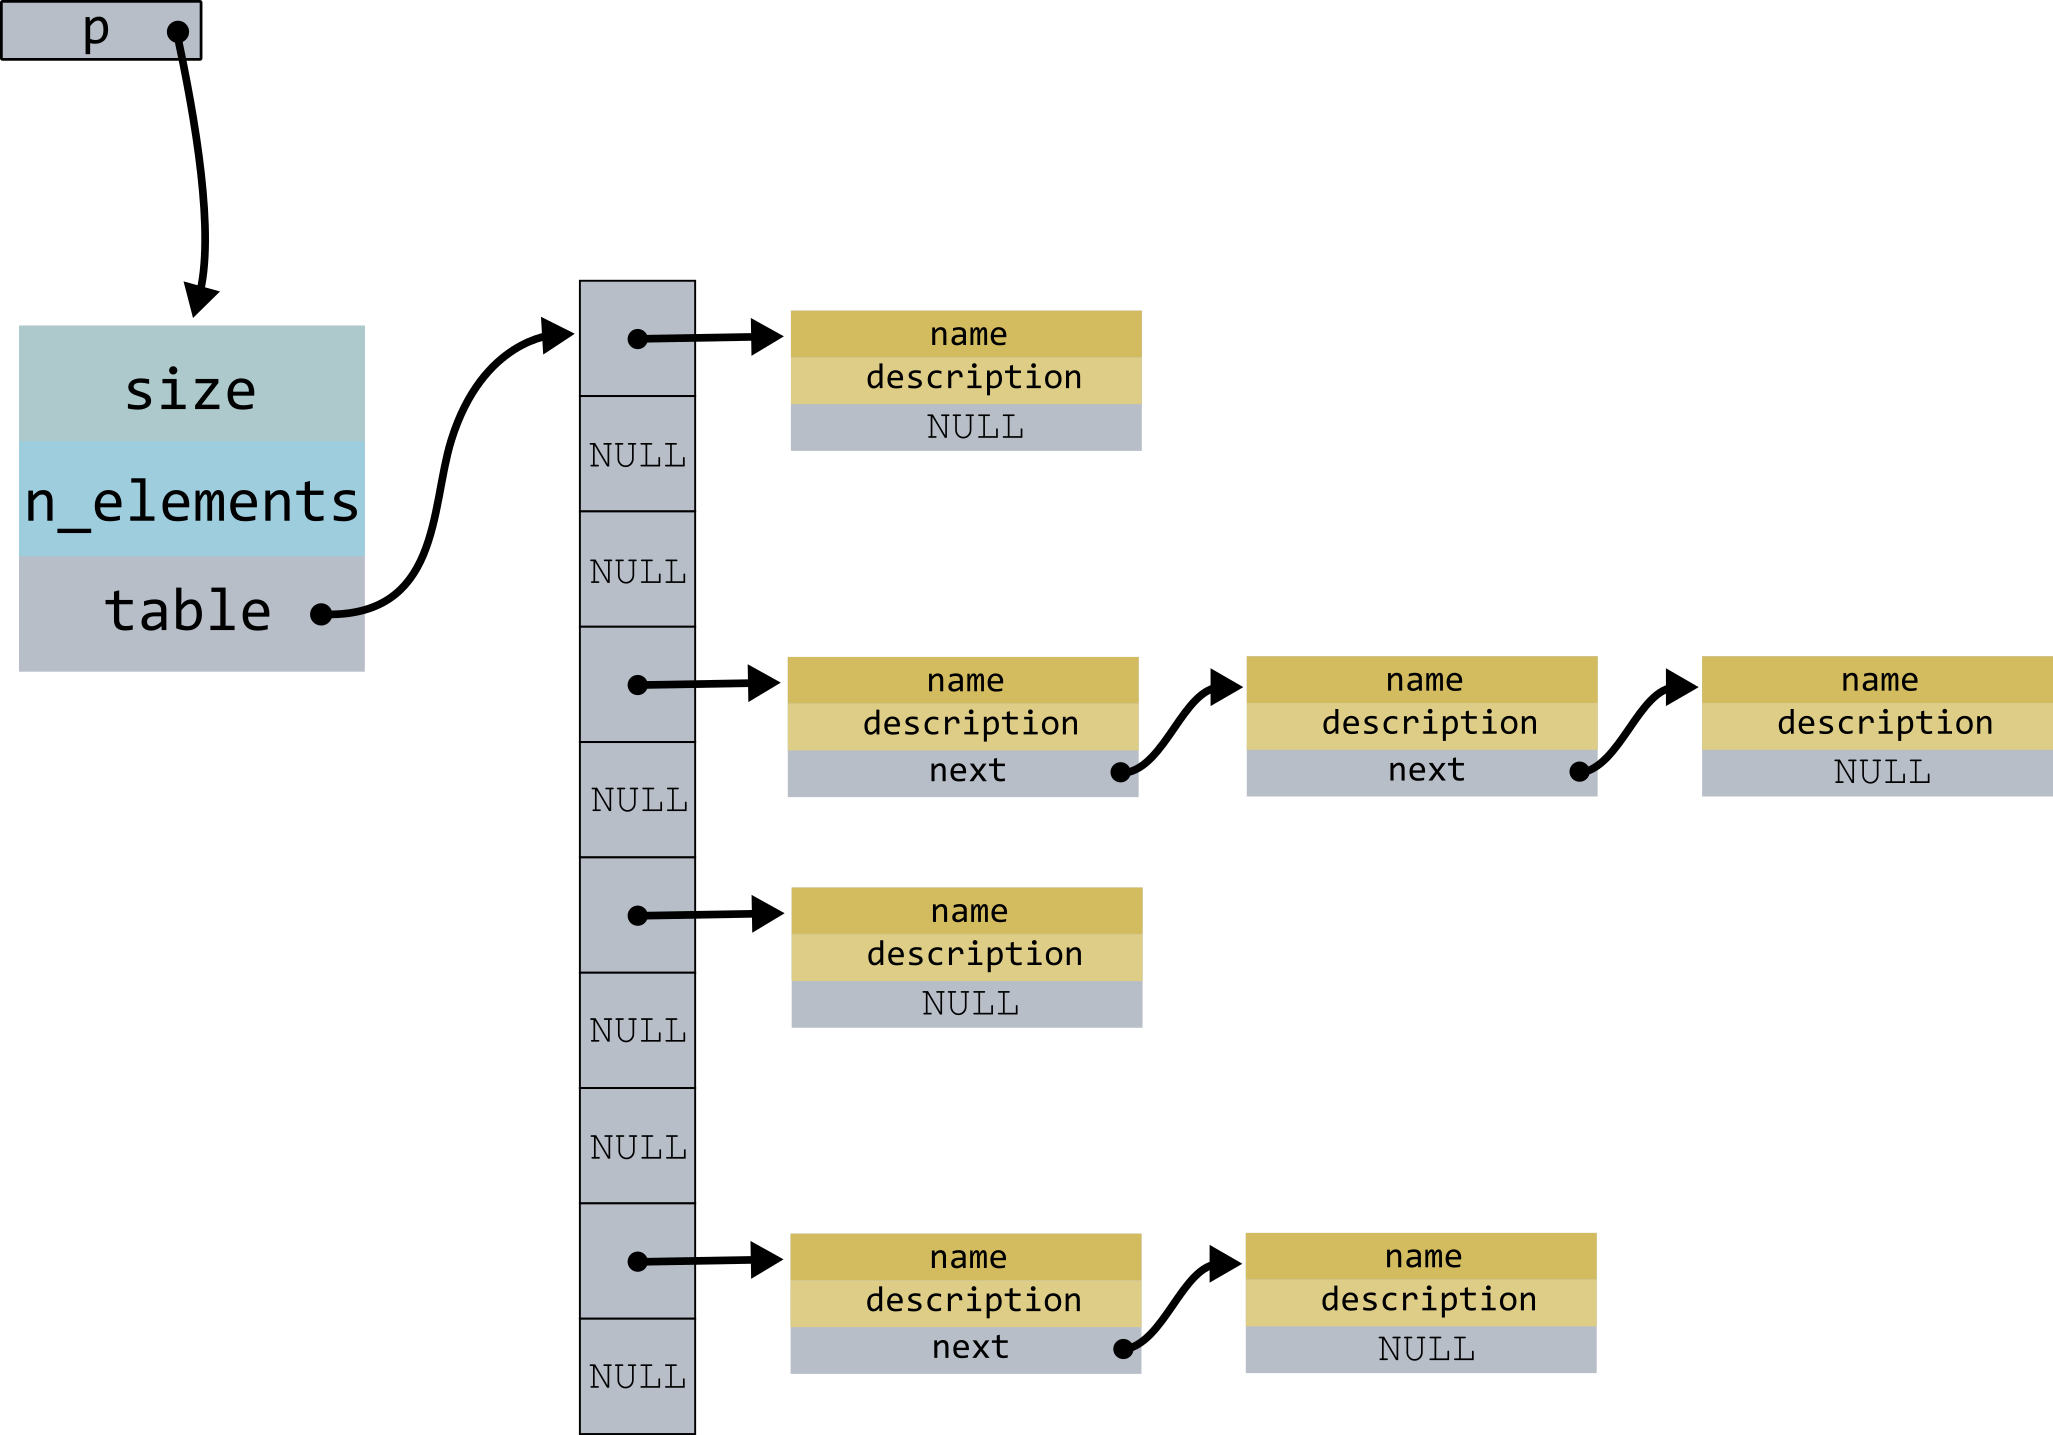
\includegraphics[scale=1.0]{../images/hashtable.png}
\end{center}

\begin{multicols}{2}
\begin{lstlisting}
struct node 
{
    char* name;
    char* description;
    struct node* next;
};
typedef struct node Node;

struct hashtable 
{
    int size;
    int n_elements;
    Node** table;
};
typedef struct hashtable Hashtable;



Hashtable* hashtable_create(int size)
{
    Hashtable* ht = malloc(sizeof(Hashtable));

    ht->size = size;
    ht->n_elements = 0;
    ht->table = malloc(sizeof(struct node *) * ht->size);

    for(int i = 0; i < ht->size; i++) 
        ht->table[i] = NULL;

    return ht;
}

\end{lstlisting}
\end{multicols}

\section*{Задачи:}
\begin{itemize}
\item Написать функцию \texttt{void hashtable\_insert(Hashtable* ht, char* name, char* description)}, которая будет добавлять пару (название города - его описание) в хеш-таблицу. Если город с таким названием в хеш-таблице уже есть, то ничего делать не надо.
\item Написать функцию \texttt{char* hashtable\_get\_description(Hashtable* ht, char* name)}, которая будет находить город по его названию. Если города нет в хеш-таблице, то эта функция должна вернуть \texttt{NULL}.
\item Написать программу, которая будет в бесконечном цикле требовать у пользователя название города и печатать его описание.
\item Написать функцию \texttt{void hashtable\_print(Hashtable* ht)}, которая будет печатать всё содержимое хеш-таблицы.
\item Написать функцию \texttt{int hashtable\_remove(Hashtable* ht, char* name)}, которая будет находить город в хеш-таблице и удалять его. Если города нет в хеш-таблице, то эта функция должна вернуть \texttt{0}, иначе - \texttt{1}.
\item Написать функцию \texttt{void hashtable\_destroy(Hashtable* ht)}, которая будет удалять все элементы хеш-таблицы и освобождать всю память.
\item Написать функцию \texttt{float get\_load\_factor(Hashtable* ht)}, которая будет вычислять фактор загруженности хеш-таблицы (среднее количество элементов в связном списке).
\item Видоизмените функцию \texttt{hashtable\_insert} так, чтобы она проверяла загруженность таблицы при каждом добавлении элемента. Если загруженность таблицы больше чем \texttt{MAX\_LOAD\_FACTOR}, то таблица должна будет вырасти в \texttt{GROWTH\_FACTOR} раз. При этом положения каждого элемента таблицы могут измениться. Проще всего создать новую таблицу и добавить туда все элементы из старой.
\item Заполните таблицу \texttt{1000000} случайными парами - название и описание. Протестируйте различные хеш-функции.
\end{itemize}
\end{document}
